\newcommand{\code}{\texttt}

\documentclass{beamer}
%\usetheme{default}
%\usetheme{Boadilla}
%\usetheme{Madrid}
\usetheme{Pittsburgh}
%\usetheme{Rochester}
%\usetheme{Copenhagen}
%\usetheme{Warsaw}
%\usetheme{Singapore}
%\usetheme{Malmoe}
%\usecolortheme{albatross}

\usepackage{pseudocode}
\usepackage{listings}

\title[RCImmix]{A Description of the RCImmix Algorithm}
\subtitle[RC]{Reference Counting with better heap allocation}
\author[N. Jervis]{Nathan Jervis}
\institute[McMaster]{
  Department of Computer Science\\
  McMaster University, Hamilton\\
  \texttt{jervisnd@mcmaster.ca}\\
  \texttt{1211159}
}


\begin{document}


%--- the titlepage frame -------------------------%
\begin{frame}[plain]
  \titlepage
\end{frame}

%--- the presentation begins here ----------------%
\begin{frame}{Overview}
	\begin{itemize}
		\item Introduction to automatic memory management
		\item Problems with existing reference counting
		\item The RCImmix algorithm
	\end{itemize}
\end{frame}

\begin{frame}{Manual Memory Management}
	\textbf{Manual Memory Management}
	\begin{itemize}
		\item Difficult to use
		\item Can cause dangling pointers
		\item Leads to memory leaks
	\end{itemize}
	\emph{Much better if the compiler/runtime can manage memory for us}
\end{frame}

\begin{frame}{Automatic Memory Management}
	\textbf{Tracing Garbage Collector:}
	\begin{itemize}
		\item Periodically pause program and follow program references
		\item Collect anything not referred to
	\end{itemize}
	\textbf{Reference Counting:}
	\begin{itemize}
		\item Counter keeps track of how many things are pointing to it
		\item When counter reaches 0, free memory
	\end{itemize}
\end{frame}

\begin{frame}{Tracing Garbage Collector}
	\textbf{Pros:}
	\begin{itemize}
		\item Is lazy about collecting
		\item Can detect and collect all forms of garbage
		\item Can compact memory to improve cache performance
	\end{itemize}
	\textbf{Cons:}
	\begin{itemize}
		\item Requires pausing the program during collection
		\item Needs complete control over the memory
	\end{itemize}
\end{frame}

\begin{frame}{Reference Counting}
	\textbf{Pros:}
	\begin{itemize}
		\item Doesn't normally stall\footnote{Can still stall a bit if large chains are freed from a single decrement, ie with large linked lists}
		\item Memory gets released at precise, defined times (as soon as they have no more references to them)
	\end{itemize}
	\textbf{Cons:}
	\begin{itemize}
		\item Poor locality (poor cache performance)
		\item Increment/Decrement for all reference copying takes a non-insignificant amount of time.
		\item Can't detect cycles
	\end{itemize}
\end{frame}


\begin{frame}{Cycles}
	\begin{center}
		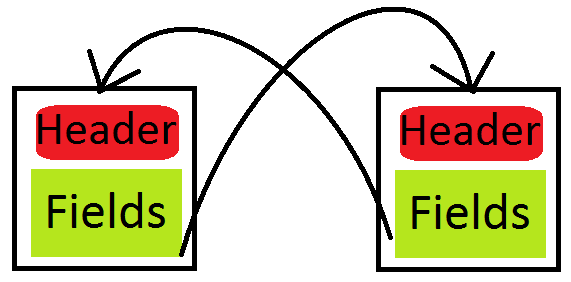
\includegraphics[width=75mm]{graphics/cycles.png}
	\end{center}
	\begin{itemize}
		\item A points to B
		\item B points to A
		\item only way A reach 0 is if B reaches 0
		\item since A points to B, B can't reach 0 until A does
		\item Reference Counting can't collect this
	\end{itemize}
\end{frame}

\begin{frame}{Initial Memory State}
	\begin{center}
		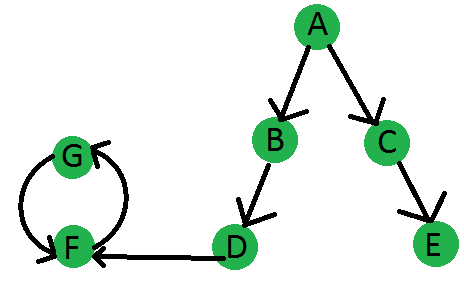
\includegraphics[width=\textwidth]{graphics/memState0.png}
	\end{center}
	\begin{itemize}
		\item Includes one cycle
		\item A is the root of the program %only one you have reference to
	\end{itemize}
\end{frame}
\begin{frame}{Initial Memory State}
	\begin{center}
		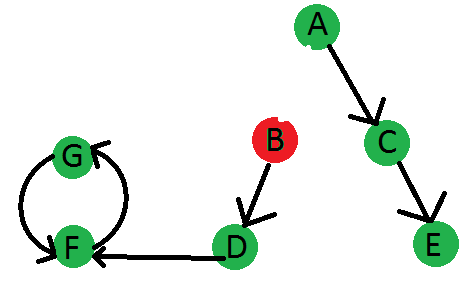
\includegraphics[width=\textwidth]{graphics/memState1.png}
	\end{center}
	\begin{itemize}
		\item A stops referring to 
		\item  B now has no references to it, and dies
	\end{itemize}
\end{frame}
\begin{frame}{Initial Memory State}
	\begin{center}
		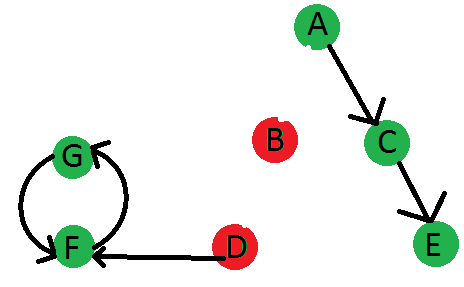
\includegraphics[width=\textwidth]{graphics/memState2.png}
	\end{center}
	\begin{itemize}
		\item B is freed, and decrements the references it's pointing to
		\item D now has no references to it, and becomes dead
	\end{itemize}
\end{frame}
\begin{frame}{Initial Memory State}
	\begin{center}
		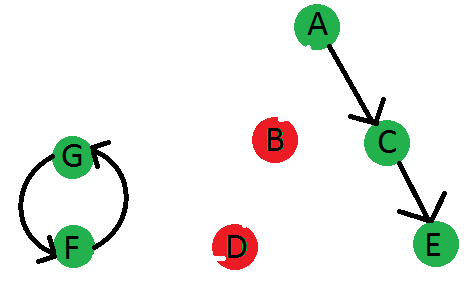
\includegraphics[width=\textwidth]{graphics/memState3.png}
	\end{center}
	\begin{itemize}
		\item D is freed, and decrements the references it's pointing to
		\item But F still has G pointing to it, so it doesn't get freed
		%Even though you can no longer access it
	\end{itemize}
\end{frame}

\begin{frame}{Block Based Memory Allocation}
	Normally memory allocation involves maintaining a list of all free locations and selecting one.\\
	
	Block based memory allocation can allocate memory within a block by simply incrementing a pointer. Example:\\
	\begin{pseudocode}{BlockAllocate}{size}
		\IF pointer + size < block.length \THEN 
			\BEGIN
				result \GETS pointer\\
				pointer \GETS pointer + size\\
			\END
		\ELSE
			\BEGIN
				block \GETS \CALL{getFreeBlock}{}\\
				pointer \GETS 0\\
			\END
	\end{pseudocode}
\end{frame}

\begin{frame}{Block Based Memory Allocation}
	\begin{itemize}
		\item With a large enough block size, the majority of calls will simply increment the pointer.
		\item Avoids expensive free list walking
		\item Also sequential calls to memory allocator will allocate memory sequentially (great for cache)
		\pause
		\item requires entire blocks to be free before any item can be used
		\pause
		\item Okay for tracing collector (can move objects)
		\pause
		\item Not usable for reference counting
	\end{itemize}
\end{frame}

\begin{frame}{Ref. Counting Problems}
	\textbf{Summary of problems with reference counting:}
	\begin{itemize}
		\item Increment/Decrement can take up non-trivial amounts of time
		\item Allocation is much more expensive than tracing collectors
		\item Poor cache performance (bad locality)
		\item Can't detect cycles
		\item Requires an entire word to store counter reliably (32 bits for every object on current machines)
	\end{itemize}
\end{frame}

\begin{frame}{Introducing RCImmix}
	\textbf{RCImmix - reference counting on steroids}
	\begin{itemize}
		\item Builds upon serious of smaller optimizations
		\item Can detect cycles
		\item Can use block-based memory allocation
		\item Much better cache performance
		\item requires only a few bits to store counter (can even use existing space in object header)
	\end{itemize}
\end{frame}

\addtocounter{section}{1}
%\section{RCImmix Description}%doesn't appear but used to correct section numbers

\begin{frame}[fragile]
\frametitle{RCImmix - How it works}
	\begin{pseudocode}{Allocate}{size}
	pointer.location \GETS \CALL{blockAllocate}{size}\\
	pointer.count \GETS 1\\
	\RETURN{pointer}
	\end{pseudocode}\\
	Make sure each time it's copied call \texttt{Retain} and each time something stops referring to it call \texttt{Release}
\end{frame}

\begin{frame}{RCImmix - How it works}
	\begin{pseudocode}{Retain}{pointer}
	\IF pointer \NOT max
		\THEN pointer.count \GETS pointer.count + 1
	\end{pseudocode}
%	\begin{pseudocode}{Release}{pointer}
		
%	\end{pseduocode}
\end{frame}

\begin{frame}{RCImmix - Cycle Collection}
	\textbf{How RC Immix deals with Cycles}
	\begin{itemize}
		\item Don't worry about cycles
		\item Will lead to unclaimed garbage
		\pause
		\item Backup tracing collector
		\item Will eventually be discovered and collected
	\end{itemize}
\end{frame}

\begin{frame}{RCImmix - Smaller counter}
	\begin{itemize}
		\item In theory: Every possible memory location could point to one spot
		\item In practice: Only a few things will ever point to it
		\item 4 bits will work for most objects
		\item If it reaches \texttt{1111} let it stay there
		\item Again leads to garbage
		\item Tracer will fix counter
	\end{itemize}
\end{frame}

\begin{frame}{RCImmix - Better cache performance}
	
\end{frame}

\end{document}